%\section{Einleitung}
\subsection{Singleton}
\begin{frame}
  \frametitle{Singleton}
  \framesubtitle{Idee}
  \begin{itemize}
    \item Klasse hat nur eine einzige Instanz
    \item Globalen Zugriffspunkt zu dieser Instanz
  
  \end{itemize}
\end{frame}

\begin{frame}
  \frametitle{Singleton}
  \framesubtitle{Pattern}
  \begin{figure}[!ht]
    \centering
    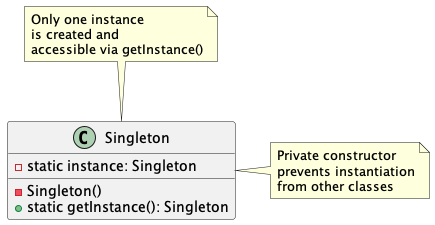
\includegraphics[width=0.65\textwidth]{fig/uml/singleton.png}
    \caption{Singleton Pattern}
    \label{fig:singleton}
  \end{figure}
\end{frame}

\begin{frame}
  \frametitle{Singleton}
  \framesubtitle{Diskussion Eignung}
  \begin{itemize}
    \item Herausforderung in VS, insbesondere bei gleichzeitigen Zugriff
    \item Nutzen spezifischen Anforderungen
    \item Manchmal sinnvoll: Zentrale Verwalten von Ressourcen und die Steuerung eines globalen Zustands
    \item Alternativen prüfen
  \end{itemize}
\end{frame}